\begin{figure}[ht]
	\centering
	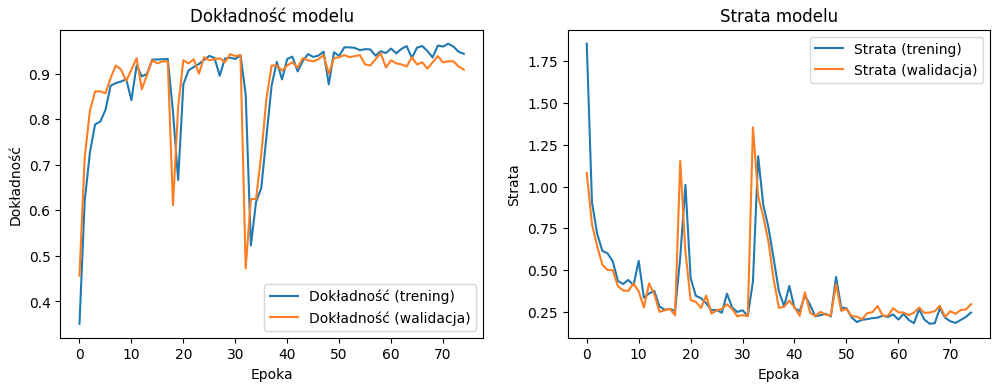
\includegraphics[height=5.5cm]{resources/tests/images/v3/base4_img.png}
	\caption{Wyniki testów dla modelu podstawowego, liczba wierzchołków = 4}
	\label{Fig:tests-base-1}
\end{figure}
\FloatBarrier

\begin{figure}[ht]
	\centering
	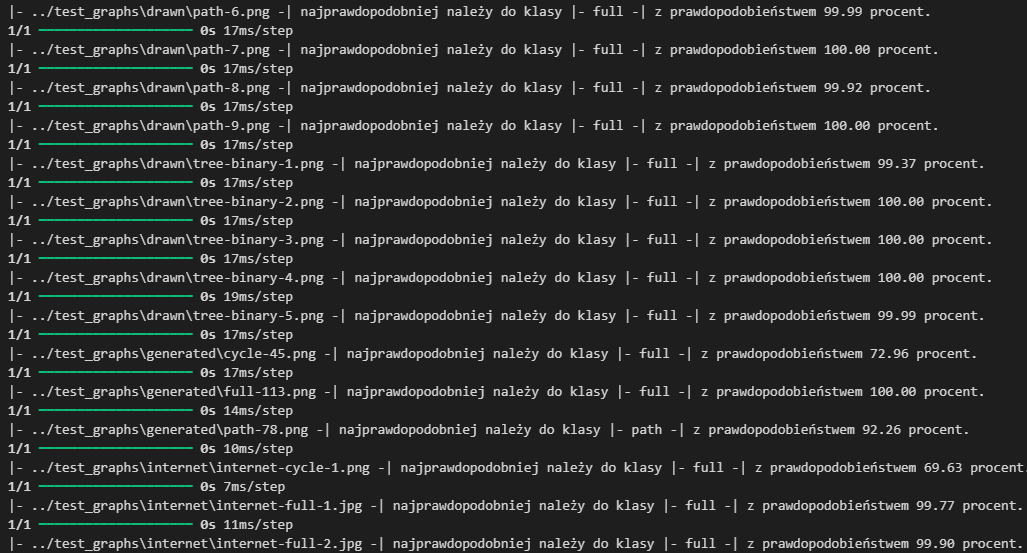
\includegraphics[height=7cm]{resources/tests/images/v3/base4_txt.png}
	\caption{Klasyfikacja obrazów zewnętrznych dla modelu podstawowego, liczba wierzchołków = 4}
	\label{Fig:tests-base-2}
\end{figure}
\FloatBarrier

\begin{figure}[ht]
	\centering
	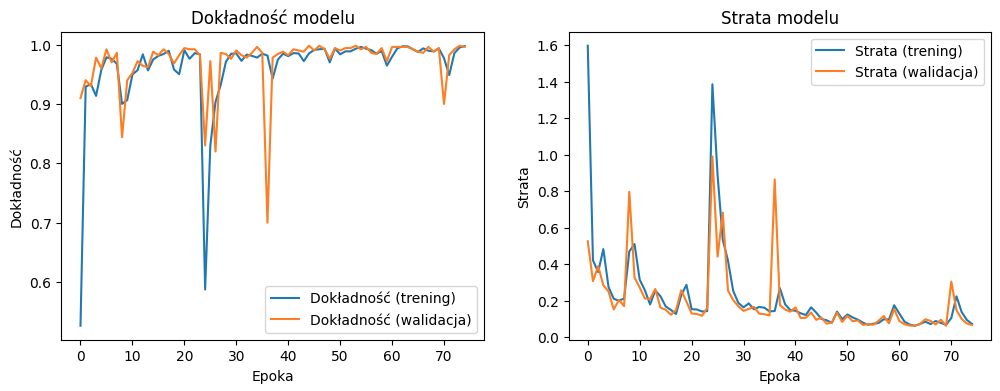
\includegraphics[height=5.5cm]{resources/tests/images/v3/base5_img.png}
	\caption{Wyniki testów dla modelu podstawowego, liczba wierzchołków = 5}
	\label{Fig:tests-base-1}
\end{figure}
\FloatBarrier

\begin{figure}[ht]
	\centering
	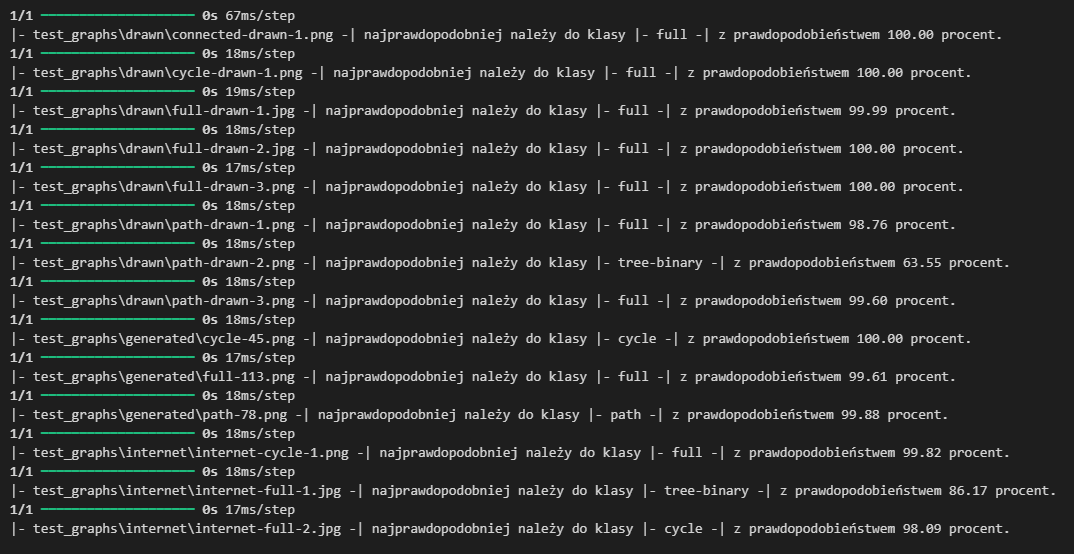
\includegraphics[height=7cm]{resources/tests/images/v3/base5_txt.png}
	\caption{Klasyfikacja obrazów zewnętrznych dla modelu podstawowego, liczba wierzchołków = 5}
	\label{Fig:tests-base-2}
\end{figure}
\FloatBarrier

\begin{figure}[ht]
	\centering
	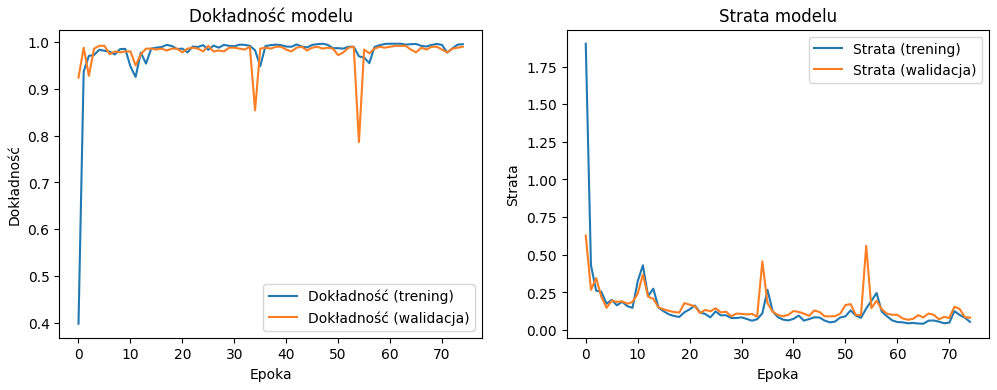
\includegraphics[height=5.5cm]{resources/tests/images/v3/base6_img.png}
	\caption{Wyniki testów dla modelu podstawowego, liczba wierzchołków = 6}
	\label{Fig:tests-base-1}
\end{figure}
\FloatBarrier

\begin{figure}[ht]
	\centering
	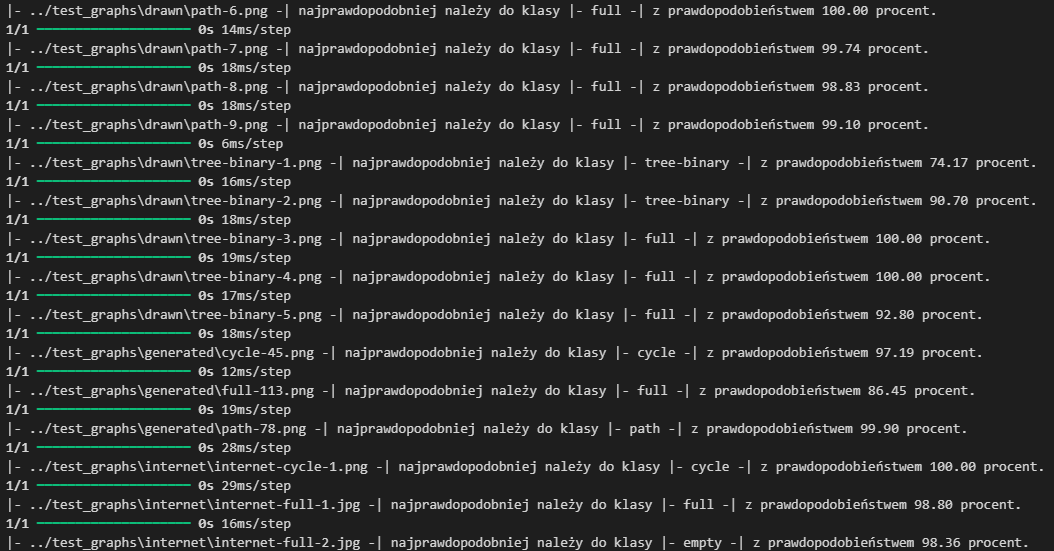
\includegraphics[height=7cm]{resources/tests/images/v3/base6_txt.png}
	\caption{Klasyfikacja obrazów zewnętrznych dla modelu podstawowego, liczba wierzchołków = 6}
	\label{Fig:tests-base-2}
\end{figure}
\FloatBarrier

\begin{figure}[ht]
	\centering
	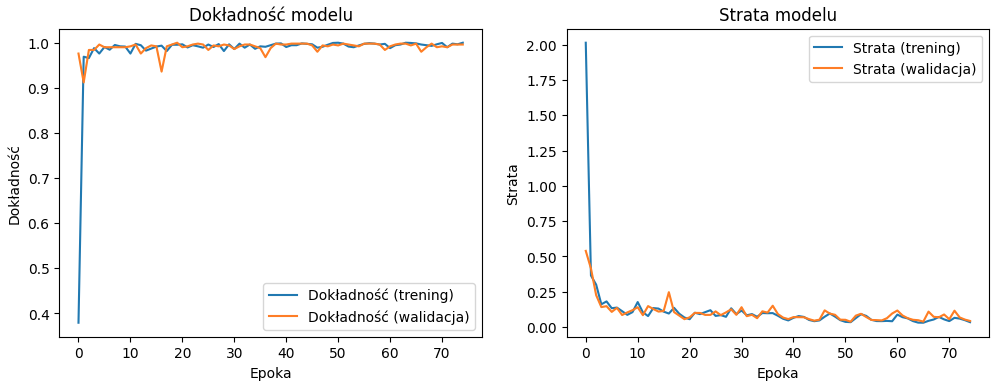
\includegraphics[height=5.5cm]{resources/tests/images/v3/base7_img.png}
	\caption{Wyniki testów dla modelu podstawowego, liczba wierzchołków = 7}
	\label{Fig:tests-base-1}
\end{figure}
\FloatBarrier

\begin{figure}[ht]
	\centering
	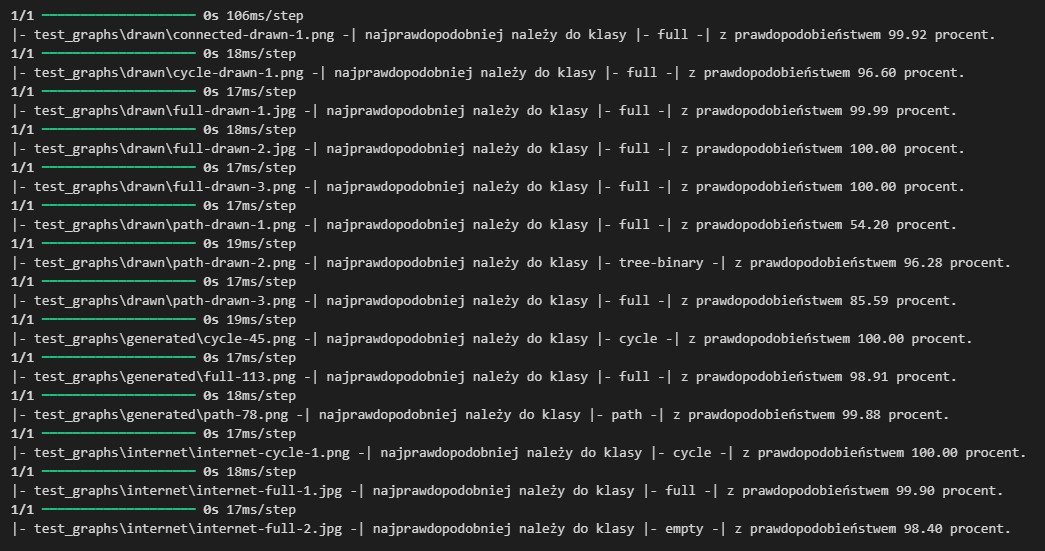
\includegraphics[height=7cm]{resources/tests/images/v3/base7_txt.png}
	\caption{Klasyfikacja obrazów zewnętrznych dla modelu podstawowego, liczba wierzchołków = 7}
	\label{Fig:tests-base-2}
\end{figure}
\FloatBarrier